\chapter{Rectas, planos y separación}
\section*{Notación}
\begin{itemize}
\item Los puntos se representan con letras mayúsculas A, B, C, etc.
\begin{center}

\begin{tikzpicture}
\draw[black] (0,0)node[]{$\bullet$} node[below]{$P$};
\end{tikzpicture}
\end{center}
\item Las rectas los denotamos por: $\mathscr{L}$ ó $\overline{AB}$.
\begin{center}
\begin{tikzpicture}
\draw[<->](0,0)--(5,0)node[right]{$\mathscr{L}  \; ó \; \overline{AB}$}; 
\draw(1,0)node[]{$\bullet$}node[below]{$A$} (4,0)node[]{$\bullet$}node[below]{$B$};
\end{tikzpicture}
\end{center}
\item Los planos se representará con letras cursivas: \textit{P}.
\end{itemize}
\begin{center}
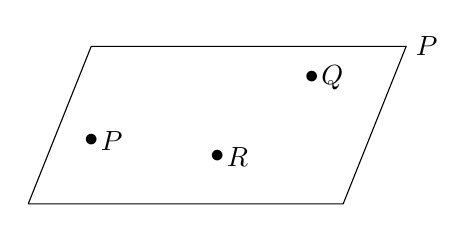
\begin{tikzpicture}[scale=0.4]
\draw(0,0)--(10,0)--(12,5)node[right]{$\mathscr{P}$}--(2,5)--(0,0);
\draw(2,2)node[]{$\bullet$}node[right]{$P$} ((6,1.5)node[]{$\bullet$}node[right]{$R$} (9,4)node[]{$\bullet$}node[right]{$Q$};
\end{tikzpicture}
\end{center}

%postulado 1
\begin{tcolorbox}[colback=black!9!,colframe=white]
\begin{post}[Postulado de la distancia] A cada par de puntos diferentes le corresponde un número real positivo único.\\
\end{post}
\end{tcolorbox}

% definición 1.1
\begin{tcolorbox}[colback=black!3!,colframe=white]
\begin{def.}
La distancia entre dos puntos es el número obtenido mediante el postulado de la distancia. Si los puntos $P$ y $Q,$ entonces indicamos la distancia por $PQ.$
\end{def.}
\end{tcolorbox}


%postulado 2
\begin{tcolorbox}[colback=black!9!,colframe=white]
\begin{post}[Postulado de la regla] Podemos establecer una correspondencia entre los puntos de una recta y los números reales de manera que:
\begin{enumerate}[\bfseries a)]
\item A cada punto de la recta corresponde exactamente un número real,
\item a cada número real corresponde exactamente un punto de la recta y
\item la distancia entre dos puntos cualesquiera es el valor absoluto de la diferencia de los números correspondientes.\\
\end{enumerate}
\end{post}
\end{tcolorbox}

%definición 1.2
\begin{tcolorbox}[colback=black!3!,colframe=white]
\begin{def.}
Una correspondencia como la descrita en el postulado de la regla se llama un sistema de coordenadas. El número correspondencia a un punto dado se llama coordenada del punto.
\end{def.}
\end{tcolorbox}

%postulado 1.3
\begin{tcolorbox}[colback=black!9!,colframe=white]
\begin{post}[Postulado de la colocación de la regla]
Dados dos puntos $P$ y $Q$ de una recta, se puede escoger el sistema de coordenadas de manera que la coordenada de $P$ sea cero y la coordenada de $Q$ sea positiva.\\
\end{post}
\end{tcolorbox}

%edfinición 1.4
\begin{tcolorbox}[colback=black!3!, colframe=white]
\begin{def.} $B$ está entre $A$ y $B$ si,
\begin{enumerate}[\bfseries i)]
\item $A,$ $B$ y $C$ son puntos distintos de una misma recta, y
\item $AB + BC = AC$\\
\end{enumerate}
\end{def.}
\end{tcolorbox}

%postulado 4
\begin{tcolorbox}[colback=black!9!,colframe=white]
\begin{post}[Postulado de la recta]
Dados dos puntos distintos cualesquiera hay exactamente una recta que los contiene.
\begin{center}
$AB$ se llama longitud del segmento $\overline{AB}$\\
\end{center}
\end{post}
Correspondencia biunivoca .- correspondencia uno a uno
\end{tcolorbox}

%definición 1.5
\begin{tcolorbox}[colback=black!3!, colframe=white]
\begin{def.}
Para dos puntos cualesquiera $A$ y $B$, el segmento $\overline{AB}$ es el conjunto de los puntos $A$ y $B$, y de todos los puntos que están entre $A$ y $B.$ Los puntos $A$ y $B$ se llaman los extremos de $\overline{AB.}$
\end{def.}
\end{tcolorbox}

%definición 1.6
\begin{tcolorbox}[colback=black!3!, colframe=white]
\begin{def.}
El número $AB$ se llama longitud del segmento $\overline{AB}$
\end{def.}
\end{tcolorbox}

%definición 1.7
\begin{tcolorbox}[colback=black!3!, colframe=white]
\begin{def.}
Sean $A$ y $B$ puntos de una recta $\mathscr{L}$ . El rayo $\overrightarrow{AB}$ es el conjunto de puntos que es la reunión de,
\begin{enumerate}
\item el segmento $\overline{AB}$ y 
\item el conjunto de todos los puntos $C$ para los cuales es cierto que $B$ está entre $A$ y $C$.
 El punto $A$ se llama el extremo de $\overrightarrow{AB}$.
\end{enumerate}
\end{def.}
\end{tcolorbox}

%definición 1.8
\begin{tcolorbox}[colback=black!3!, colframe=white]
\begin{def.}
Si $A$ está entre $B$ y $C$, entonces $\overrightarrow{AB}$ y $\overrightarrow{AC}$ se llaman rayos opuestos.
\end{def.}
\end{tcolorbox}

%teorema 1.1
\begin{teo}[Teorema de la localización de puntos] Sea $\overrightarrow{AB}$
un rayo y sea $x$un número positivo. Entonces existe exactamente un punto $P$ de $\overrightarrow{AB}$ tal que $AP=x$ \\\\
Demostración.- \; Dada la recta $\overleftrightarrow{AB}$; por el postulado de la colocación de la regla podemos elegir un sistema de coordenadas donde $A$ sea cero y la coordenada de $B$ sea un número positivo $r$
\begin{center}
\begin{tikzpicture}[scale=1]
\tkzDefPoints{0/0/A,5/0/B,8/0/P}
\tkzDefPoints{0/0/0,5/0/r,8/0/x}
\tkzDrawLine[<->](0,x)
\tkzLabelPoints(0,r,x)
\tkzDrawPoints(A,B,P)
\tkzLabelPoints[above](A,B,P)
\end{tikzpicture}
\end{center}
Sea $P$ el punto cuyo coordenada es $x$; como $x\in \mathbb{R}^+$ entonces $x\in \overrightarrow{AB}$ y $AP=|x-0|=x$. La unicidad de $P$ se da por el postulado de la regla.\\\\
\end{teo}

%definición 1.9
\begin{tcolorbox}[colback=black!3!,colframe=white]
\begin{def.}
Un punto $B$ se llama punto medio de un segmento $\overline{AC}$, si $B$ está entre $A$ y $C$ tal que $AB=BC$\\
\begin{center}
Decimos que el punto medio de un segmento \textbf{biseca} al segmento. \\
\end{center}
\end{def.}
\end{tcolorbox}

%teorema 1.2
\begin{teo}
Todo segmento tiene exactamente un punto medio.\\\\
Demostración.- \; Si $B$ es el punto medio de $\overline{AC}$ entonces debe cumplirse: 
\begin{center}
$\left.
\begin{array}{rcl}
AB + BC & = & AC\\ 
AB & = & BC
\end{array}
\right\}
\Rightarrow AB = \dfrac{AC}{2}$
\end{center}
Luego por teorema, el rayo $\overrightarrow{AC}$ con $x=\dfrac{AC}{2} \in \mathbb{R}^+$ hay exactamente un punto $B$ tal que $AB=\dfrac{AC}{2}$. Así $\overline{AC}$ tiene exactamente un punto medio.\\\\ 
\end{teo}

%definición 1.10
\begin{tcolorbox}[colback=black!3!,colframe=white]
\begin{def.}
Decimos que el punto medio de un segmento biseca al segmento.
\end{def.}
\end{tcolorbox}

%definición 1.11
\begin{tcolorbox}[colback=black!3!,colframe=white]
\begin{def.}
El conjunto de todos los puntos se llama espacio.
\end{def.}
\end{tcolorbox}

%definición 1.12
\begin{tcolorbox}[colback=black!3!,colframe=white]
\begin{def.}
Los puntos de un conjunto están alineados o son colineales, si hay una recta que los contiene a todos.
\end{def.}
\end{tcolorbox}

%definición 1.13
\begin{tcolorbox}[colback=black!3!,colframe=white]
\begin{def.}
Los puntos de un conjunto son coplanarios si hay un plano que los contiene a todos.
\end{def.}
\end{tcolorbox}

\section{Repaso del capítulo 2}
\begin{enumerate}[\bfseries \Large 1.]
%-----------------------------1------------------------------------------
\item Sea $A$ el conjunto de todos los meses del año cuyos nombres empiezan con la letra $J$.\\
Sea $B$ el conjunto de todos los meses del año que tienen exactamente 30 días.\\
Sea $C$ el conjunto de todos los meses del año cuyos nombres empiezan con la letra $F$.
\begin{enumerate}[\bfseries (a)]
%(a)
\item ¿Cuál es la intersección de $A$ y $C$? \\\\
Respuesta.- \; Conjunto vació.\\\\
%(b)
\item ¿Cuál es la reunión de $A$ y $C$?\\\\
Respuesta.- \; $A \cup C = \lbrace febrero, \; junio, \; julio \rbrace$\\\\
%(c)
\item ¿Cuál es la intersección de $B$ y $C$?\\\\
Respuesta.- \; Conjunto vació.\\\\
%(d)
\item ¿Es $C$ un subconjunto del conjunto $A$? ¿Del conjunto $B$? ¿Y del conjunto $C$?\\\\
Respuesta.- \; $C$ no es subconjunto de $A$. $C$ no es subconjunto de $B$. $C$ es subconjunto de $C$\\\\
\end{enumerate}

%-------------------------------2--------------------------------------------
\item .

\begin{center}
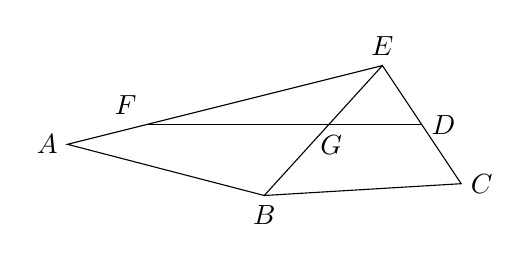
\begin{tikzpicture}[scale=0.5]
\draw(0,0.7)node[below]{$B$}--(5,1)node[right]{$C$}--(3,4)node[above]{$E$}--(0,0.7)--(-5,2)node[left]{$A$}--(3,4);
\draw(-3,2.5)node[above left]{$F$}--(4,2.5)node[right]{$D$};
\draw(1.7,1.5)node[above]{$G$};
\end{tikzpicture}
\end{center}

\begin{enumerate}[\bfseries (a)]
%(a)
\item ¿Cuál es la intersección de $\overline{FD}$ y $\overline{BE}$?\\\\
Respuesta.- \; $G$\\\\

%(b)
\item ¿Cuál es la intersección de $\overline{AE}$ y el triángulo $FGE$?\\\\
Respuesta.- \; $\overline{FE}$\\\\

%(c)
\item ¿Cuál es la reunión de $\overline{ED}$ y $\overline{DC}$?\\\\
Respuesta.- \; $\overline{EC}$\\\\

%(d)
\item ¿Cuál es la reunión de $\overline{BG}$ y $\overline{BE}$?\\\\
Respuesta.- \; $\overline{BE}$\\\\

%(e)
\item ¿Cuál es la intersección de $\overline{AB}$ y $\overline{EG}$?\\\\
Respuesta.- \; Conjunto vació.\\\\
\end{enumerate}

%----------------------------------3------------------------------------
\item 
\begin{enumerate}[\bfseries (a)]
%(a)
\item ¿Cuántos cuadrados tiene un número positivo dado?\\\\
Respuesta.- \; Uno\\\\ 

%(b)
\item ¿Cuál es el cuadrado de $4$?\\\\
Respuesta.- \; Dos\\\\

%(c)
\item ¿Cuántas raices cuadradas tiene un número positivo dado?\\\\
Respuesta.- \; Dos\\\\

%(d)
\item ¿Es $\sqrt{4}$ negativo?\\\\
Respuesta.- \; Si, ya que $-2^2 $ es $2$ de las misma forma que $2^2$\\\\
\end{enumerate}

%------------------------------4-----------------------------------------
\item Expresar los siguientes números sin el símbolo de valor absoluto:
\begin{enumerate}[\bfseries (a)]
\item $|-6| = 6$
\item $|5-7| = 2$
\item $|5|-|7| = -2$
\item $|-5| = 5$
\item $|n| = n$
\item $|-n| = n$
\item $|n+(-n)| = 0$
\item $|n| + |-n| = 2n$\\\\
\end{enumerate}

%-----------------------------------5-------------------------------
\item 
\begin{enumerate}[\bfseries (a)]
\item Si $a<b$, entonces $a-b$ es \textbf{Negativo}
\item Si $a=b$, entonces $a-b$ es \textbf{Cero}
\item Si $a>b$, entonces $a-b$ es \textbf{Positivo}\\\\
\end{enumerate}

%---------------------------------6----------------------------------
\item .
\begin{center}
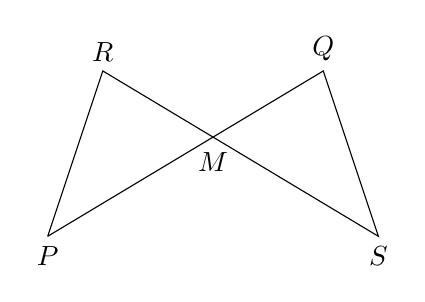
\begin{tikzpicture}[scale=.7]
\draw(0,0)node[below]{$P$}--(5,3)node[above]{$Q$}--(6,0)node[below]{$S$}--(1,3)node[above]{$R$}--(0,0);
\draw(3,1)node[above]{$M$};
\end{tikzpicture}
\end{center}
\begin{enumerate}[\bfseries (a)]
%(a)
\item ¿Qué ecuación define posiciones relativas de los puntos $P$, $M$ y $Q$?\\\\
Respuesta.- \; $\overline{PQ}$\\\\

%(b)
\item ¿En qué condiciones sería $M$ el punto medio de $\overline{RS}$?\\\\
Respuesta.- \; Un punto $M$ se llama punto medio de un segmento $\overline{RS}$, si $M$ está entre $R$ y $S$ y $RM=MS$\\\\
\end{enumerate}

%-------------------------------7------------------------------------------
\item Cuatro puntos $A$, $B$, $C$ y $D$ se disponen a lo largo de una recta de manera que $AC>AB$ y $BD<BC$. Hacer un dibujo de los cuatro puntos colocados de la manera indicada. ¿Habrá más de un orden posible? Explíquese.\\\\
Respuesta.- \; 

%----------------------------------8------------------------------------
\item $G$ es el conjunto de todos los pares de números enteros $x$ é $y$ cuya suma es $21$. $H$ es el conjunto de todos los pares de números enteros $x$ é $y$ cuya diferencia es $5$.
\begin{enumerate}[\bfseries (a)]
%(a)
\item ¿Pertenece a $G$ el par $15$ y $6$?\\\\
Respuesta.- \; Efectivamente ya que $15+6=21$\\\\

%(b)
\item ¿Pertenece a $H$ el par $9$ y $4$?\\\\
Respuesta.- \; Efectivamente ya que $9-4=5$\\\\

%(c)
\item ¿Cuál es la intersección de $G$ y $H$?\\\\
Respuesta.- \; El par $13$ y $8$ ya que $13+8=21$ y $13-8=5$\\\\
\end{enumerate}

%----------------------------------9--------------------------------
\item .
\begin{center}
\begin{tikzpicture}[scale=1]
\tkzDefPoints{-4/0/P,-3/0/Q,-2/0/R,-1/0/S,0/0/T,1/0/U,2/0/V,3/0/W,4/0/X,5/0/Y,6/0/Z}
\tkzDefPoints{-4/0/-4,-3/0/-3,-2/0/-2,-1/0/-1,0/0/0,1/0/1,2/0/2,3/0/3,4/0/4,5/0/5,6/0/6}
\tkzDrawLine[<->](-4,6)
\tkzLabelPoints[above](P,Q,R,S,T,U,V,W,X,Y,Z)
\tkzDrawPoints(P,Q,R,S,T,U,V,W,X,Y,Z)
\tkzLabelPoints[below](-4,-3,-2,-1,0,1,2,3,4,5,6)
\end{tikzpicture}
\end{center}
\begin{enumerate}[\bfseries (a)]
%(a)
\item ¿Cuál es la coordenada de $W$? ¿y la de $S$?\\\\
Respuesta.- \; La coordenada de $W$ es $3$ y la de $S$ es $-1$\\\\
%(b)
\item ¿cuál es el nombre del punto cuya coordenada es $0$? ¿cuya coordenada es $-3$?\\\\
Respuesta.- \; El nombre de $0$ es $T$ y de $-3$ es $Q$\\\\
%(c)
\item ¿Evaluar $RT$ ,$VZ$ ,$TW$ ,$TQ$, $RW$, $PZ$, $XS$, $YQ$?\\\\
Respuesta.- \; 
\begin{center}
\begin{tabular}{r c l c l}
$RT$&$=$&$|-2-0|$&$=$&$2$\\
$VZ$&$=$&$|2-6|$&$=$&$4$\\
$TW$&$=$&$|0-3|$&$=$&$3$\\
$TQ$&$=$&$|0-(-3)|$&$=$&$3$\\
$RW$&$=$&$|-2-3|$&$=$&$5$\\
$PZ$&$=$&$|-4-6|$&$=$&$10$\\
$XS$&$=$&$|4-(-1)|$&$=$&$5$\\
$YQ$&$=$&$|5-(-3)|$&$=$&$8$\\\\
\end{tabular}
\end{center}
\end{enumerate}
%---------------------------10--------------------------------
\item Se da un sistema de coordenadas en una recta. La coordenada de $A$ es $6$, la de $B$ es $-2$, la de $C$ es $1$, la de $D$ es $x$ y la de $E$ es $y$.
\begin{enumerate}[\bfseries (a)]
%(a)
\item ¿Qué punto tiene, que estar entre otros dos puntos, y cuáles son estos?\\\\
Respuesta.- \; La coordenada $C$ esta entre las coordenadas $B$ y $A$\\\\
%(b)
\item Evaluar $AB$, $BC$, $AD$, $CE$, $BE$, $DE$\\\\
Respuesta.- \; 
\begin{center}
\begin{tabular}{r c l c l}
$AB$&$=$&$|6-(-2)|$&$=$&$8$\\
$BC$&$=$&$|-2-1|$&$=$&$3$\\
$AD$&$=$&$|6-x|$&&\\
$CE$&$=$&$|1-y|$&&\\
$BE$&$=$&$|-2-y|$&&\\
$DE$&$=$&$|x-y|$&&\\\\
\end{tabular}
\end{center}
%(c)
\item Si $x-6>0$ y $y-(-2)<0,$ ¿en qué orden están dispuestos los cinco puntos en la recta?\\\\
Respuesta.- \; El orden en que se disponen es $y$, $B$, $C$, $A$, $x$\\\\
\end{enumerate}

%---------------------------11--------------------------------
\item Se da un sistema de coordenadas en una recta. La coordenada de $P$ es $7$ y la coordenada de $Q$ es $-12$ ¿Cuál es la coordenada de $M$, si $MP=MQ$?\\\\
Respuesta.- \; Decimos que la distancia entre $PQ $ es $19$, entonces la coordenada $M$ es $\dfrac{19}{2} = 9.5$\\\\

%-----------------------------12-------------------------------
\item Indicar si cada uno de los siguientes enunciados es cierto o falso.
\begin{enumerate}[\bfseries (a)]
%(a)
\item $-5$ es un entero.\\\\
Respuesta.- \; Cierto.\\\\

%(b)
\item $\dfrac{4}{7}$ es un número real.\\\\
Respuesta.- \; Cierto.\\\\

%(c)
\item $0$ es un número racional.\\\\
Respuesta.- \; Cierto.\\\\

%(d)
\item $\sqrt{8}$ es un número racional.\\\\
Respuesta.- \; Falso.\\\\

%(e)
\item $\sqrt{9}$ es un entero.\\\\
Respuesta.- \; Cierto. \\\\

%(f)
\item $- \dfrac{31}{6}$ es un número racional.\\\\
Respuesta.- \; Cierto. \\\\

%(g)
\item $\dfrac{\sqrt{2}}{4}$ es un número racional.\\\\
Respuesta.- \; Falso.\\\\.\\\\

%(h)
\item $-x$ es un número negativo para todo número real $x$. \\\\
Repuesta.- \; Falso.\\\\

%(i)
\item $- \sqrt{\dfrac{4}{9}}$ es un número racional.\\\\
Respuesta.- \; Cierto.\\\\

%(j)
\item $|x|=x$. \\\\
Respuesta.- \; Falso.\\\\
\end{enumerate}

%--------------------------13---------------------------
\item Si la distancia de $A$ a $B$, medida en centímetros, es $k$, ¿cuál será la distancia $AB$ medida en metros?\\\\
Respuesta.- \; La distancia de $AB$ es $\dfrac{k}{60}$\\\\

%-------------------------14------------------------------
\item Si la distancia de $P$ a $M$, medida en yardas, es $t,$ ¿Cuánto es $PM$, en pulgadas?\\\\
Respuesta.- \; $PM=t\cdot 36$\\\\

%-------------------------15---------------------------------
\item Los pares de letras en el siguiente párrafo representan o bien números, o retas, o segmentos de recta o rayos. Copiar el párrafo, colocando los símbolos apropiados.\\\\
Respuesta.- \; $\overline{AB}+\overline{BC}=\overline{AC}$.  $\overrightarrow{DB}$ contiene a los puntos $A$ y $C$,  pero $DB$ no contiene ni el punto $A$ ni el punto $C.$ $A$ pertenece a $\overline{DB}$, pero $C$ no.

\begin{center}
\begin{tikzpicture}
\tkzDefPoints{0/0/D,2/0/A,4/0/B,6/0/C}
\tkzDrawLine[<->](0,6)
\tkzDrawPoints(A,B,C,D)
\tkzLabelPoints[below](A,D,B,C)
\end{tikzpicture}
\end{center} 
\vspace{0.5cm}

%-------------------------16---------------------------------
\item Si $A,B,C$  y $D$ son puntos distintos tales que $\overleftrightarrow{AC}$ contiene a $B$ y $\overleftrightarrow{BD}$ contiene a $C$, ¿Cuáles de los siguientes enunciados tienen que ser ciertos?
\begin{enumerate}[\bfseries (a)]
%(a)
\item $B$ está entre $A$ y $C$.\\\\
Respuesta.- \; Cierto.\\\\ 

%(b)
\item $\overleftrightarrow{BC}$ contiene a $A$\\\\
Respuesta.- \; Cierto\\\\

%(c)
\item $\overleftrightarrow{AC} = \overleftrightarrow{BD}$\\\\
Respuesta.- \; Falso \\\\

%(d)
\item $\overleftrightarrow{AC} y \overleftrightarrow{BD}$ se intersecan en $B$ y $C$ solamente.\\\\
Respuesta.- \; Falso\\\\

%(e)
\item $\overleftrightarrow{AD}$ y $\overleftrightarrow{BC}$ no se intersecan.\\\\
Respuesta.- \; Falso\\\\

%(f)
\item $\overleftrightarrow{AC}$ es opuesto a $\overleftrightarrow{DB}$\\\\
Respuesta.- \; Falso\\\\
\end{enumerate}

%-------------------------17---------------------------------
\item Se da un sistema de coordenadas en $\overleftrightarrow{AB}$ tal que $\overline{AB}$ es el conjunto de todos los puntos cuyas coordenadas $x$ satisfacen la condición $-5\leq x \leq 7$. La coordenada de $A$ es menor que la coordenada de $B$.
\begin{enumerate}[\bfseries (a)]
%(a)
\item ¿Cuál es la coordenada del extremo de $\overrightarrow{AB}$? ¿Del extremo de $\overrightarrow{BA}$? ¿Y del extremo del rayo opuesto a $\overrightarrow{BA}$?\\\\
Respuesta.- \; La coordenada del extremo de $\overrightarrow{AB}$ es $-5\leq x \leq \infty$, del extremo de $\overrightarrow{BA}$ es $- \infty \leq x \leq 7$, y del extremo del rayo opuesto a $\overrightarrow{BA}$ es $7 \leq x \leq \infty$\\\\

%(b)
\item Cuál es la coordenada del punto medio de $\overline{AB}$\\\\
Respuesta.- \; Es 6.\\\\
\end{enumerate}

%-------------------------18---------------------------------
\item  \begin{enumerate}[\bfseries (a)]
%(a)
\item Dibujar dos segmentos $\overline{AB}$ y $\overline{CD}$ para los cuales la intersección de $\overline{AB}$ y $\overline{CD}$ es el conjunto vacío, pero la intersección de $\overleftrightarrow{AB}$ y $\overleftrightarrow{CD}$ es exactamente un punto.\\\\
Respuesta.- \; 
\begin{center}
\begin{tikzpicture}
\tkzDefPoints{1/0/C,5/0/D}
\tkzDrawLine[<->](0,6)
\tkzDrawPoints(C,D)
\tkzLabelPoints[below](C,D)
\vspace{0.5cm}
\end{tikzpicture}
\end{center}

%(b)
\item Dibujar dos segmentos $\overline{PQ}$ y $\overline{RS}$ para los cuales la intersección de $\overline{PQ}$ y $\overline{RS}$ es el conjunto vacío, pero $\overleftrightarrow{PQ} = \overleftrightarrow{RS}$\\\\
Respuesta.- \;  
\end{enumerate}

%-------------------------19---------------------------------
\item La primera numeración de los puntos de la recta siguiente representa un sistema de coordenadas. Basándose en el postulado de la regla y en el postulado de colocación de la regla, determinar cuáles de las numeraciones dadas en $(a)$ a $(e)$ no representan sistemas de coordenadas.
\begin{center}
\begin{tikzpicture}[scale=1]
\tkzDefPoints{-4/0/P,-3/0/Q,-2/0/R,-1/0/S,0/0/T,1/0/U,2/0/V,3/0/W,4/0/X,5/0/Y,6/0/Z}
\tkzDefPoints{-4/0/-4,-3/0/-3,-2/0/-2,-1/0/-1,0/0/0,1/0/1,2/0/2,3/0/3,4/0/4,5/0/5,6/0/6}
\tkzDrawLine[<->](-4,6)
\tkzDrawPoints(P,Q,R,S,T,U,V,W,X,Y,Z)
\tkzLabelPoints[below](-4,-3,-2,-1,0,1,2,3,4,5,6)
\end{tikzpicture}
\end{center}

\begin{center}
\begin{tabular}{c c c c c c c c c c c c l}
(a)&-4&3&2&1&0&-1&-2&-3&-4&-5&-6&\\
(b)&-6&-5&-4&-3&-2&-1&0&1&2&3&4&\\
(c)&0&1&2&3&4&5&6&7&8&9&0&\\
(d)&-10&-9&-8&-7&-6&-5&-4&-3&-2&-1&0&\\
(e)&5&4&3&2&1&0&1&2&3&4&5&\\\\
\end{tabular}
\end{center}

%-------------------------20---------------------------------
\item Para cada uno de los siguientes enunciado, considerar el conjunto de puntos de una recta cuyas coordenadas $x$ satisfacen la condición dada:
\begin{enumerate}[\bfseries (a)]
\item $x\leq 3$
\item $x=1$
\item $5 \geq x \geq 0$
\item $x \geq 1$
\item $x = -4$
\item $x \leq -2$ ó $x \geq 2$
\item $|x| \leq 2$
\item $|x| \geq 0$
\end{enumerate}
¿Cuáles de los conjuntos es un rayo? ¿un punto?, ¿una recta?, ¿y un segmento?. Hacer un dibujo de cada una de las figuras.

\end{enumerate}






%postulado 5
\begin{tcolorbox}[colback=black!9!,colframe=white]
\begin{post}(Postulado de la Existencia de puntos).
\begin{enumerate}[\bfseries a)]
\item Todo plano contiene al menos tres puntos no colineales.
\item El espacio existe y contiene por lo menos, cuatro puntos no son coplanares.
\item Una recta contiene, por lo menos dos puntos.
\end{enumerate}
\end{post}
\end{tcolorbox}

%teorema 3
\begin{teo}
Si dos rectas diferentes se intersecan, su intersección contiene un punto solamente.\\\\
Demostración.- \; (contradicción). \\
El teo. expreso: 
\begin{center}
Si las rectas $\mathscr{L}_1$ y $\mathscr{L}_2$ se intersecan entonces existe exactamente un punto $P$ tal que $\mathscr{L}_1 \cap \mathscr{L}_2 = \lbrace P \rbrace$
\end{center}
empleando el método de la contradicción; afirmamos $\mathscr{L}_1 \;  y \; \mathscr{L}_2$, $\mathscr{L}_1 \neq \mathscr{L}_2$ se intersecan y su intersección contiene dos puntos $P$ y $Q$
Un gráfico de la afirmación (absurda) es:


\begin{center}
\begin{tikzpicture}

\end{tikzpicture}
\end{center}


Si $\mathscr{L}_1 \;  y \; \mathscr{L}_2$ se intersecan en los puntos $P$ y $Q$ entonces por los puntos $P$ y $Q$ pasan las rectas $\mathscr{L}_1$ y $\mathscr{L}_2$; lo que es una contradicción al postulado de la recta.
\begin{center}
$\therefore$ La afirmación del teorema es verdad.
\end{center}
\end{teo}

%postulado 6
\begin{tcolorbox}[colback=black!9!,colframe=white]
\begin{post}[Postulado de los dos Puntos de la Recta y el Plano] Si dos puntos están en un plano, entonces la recta que los contiene esta en el mismo plano.
\end{post}
\end{tcolorbox}

%teorema 4
\begin{teo}
Si una recta interseca a un plano que no la contiene, entonces la intersección contiene un solo punto.\\\\
Demostración.- \; (Contradicción)\\
Suponemos $ \mathscr{L} \not\subset \mathscr{P}$ y $\mathscr{L} \cap \mathscr{P} = \lbrace P,Q \rbrace$\\
Si $P,Q \in \mathscr{P}$ \; y \; $P,Q \in \mathscr{L}$ entonces por postulado 6 $\mathscr{L} \subset \mathscr{P} \; ( \Rightarrow \Leftarrow)$ 
\begin{center}
\begin{tikzpicture}

\end{tikzpicture}
\end{center} 
\end{teo}

%postulado 7
\begin{tcolorbox}[colback=black!9!,colframe=white]
\begin{post}[Postulado del Plano] Tres puntos cualesquiera están al menos en un plano, y tres puntos cualesquiera no alineados están exactamente en un plano.
\end{post}
\end{tcolorbox}

%teorema 5
\begin{teo}
Dada una recta y un punto fuera de ella, hay exactamente un plano que contiene a ambos.\\\\
Demostración.- \; El teorema afirma: 
\begin{center}
Si $P \not\subset \mathscr{L} \Rightarrow \exists ! \mathscr{P} / P \in \mathscr{P}$ y $\mathscr{L} \subset \mathscr{P}$\\
\begin{tikzpicture}

\end{tikzpicture}
\end{center}
Por el postulado 5 inciso c) $\mathscr{L}$ contiene al menos dos puntos $R$ y $S$; luego $P,R$ y $S$ son no alineados y por el postulado 7 $P,R$ y $S$ están exactamente en un plano $\mathscr{P};$ además como $R,S \in \mathscr{L}$ entonces por el postulado 6 $\mathscr{L} \subset \mathscr{P}$\\\\
\end{teo}

%teorema 6
\begin{teo}
Dados dos rectas que se intersecan, hay exactamente un plano que las contiene.\\\\
Demostración.- \;  
$$ \mathscr{L}_1 \; y \; \mathscr{L}_2 \; \mbox{son dos rectas y se intersecan en el punto}\;  P \:, entonces \; \exists! \; P \; / \; \mathscr{L}_1 \subset E \; y \; \mathscr{L}_2 \subset E $$
\begin{center}
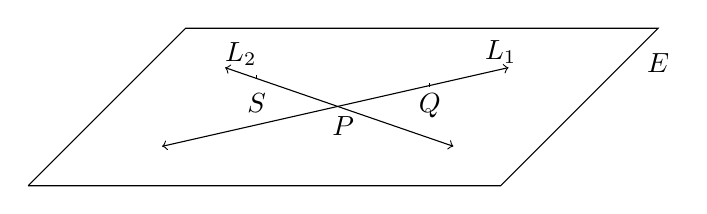
\begin{tikzpicture}
\draw[<->] (1.7,0.5) -- (6.1,1.5);
\draw[<->] (5.4,0.5) -- (2.5,1.5);
\draw (0,0) -- (2,2) -- (8,2) -- (6,0) -- (0,0) ;
\draw (8,1.8) node[below] {$\mathscr{E}$};
\draw (6,1.43) node[above] {$\mathscr{L}_1$};
\draw (2.7,1.4) node[above] {$\mathscr{L}_2$};
\draw (4,1) node[below] {$P$};
\draw (5.1,1.3) node[below] {$Q$};
\draw (5.1,1.3) -- (5.1,1.25);
\draw (2.9,1.3) node[below] {$S$};
\draw (2.9,1.4) -- (2.9,1.35);

\end{tikzpicture}
\end{center}
Por el postulado de la recta consideramos los puntos $Q,P \in \mathscr{L}_1 $ y $S,P \in \mathscr{L}_2$, así por hipótesis y teorema 3 podemos decir que $P$ interseca a las dos rectas. Luego si $Q \in \mathscr{L}_1$ y $S \in \mathscr{L}_2$ entonces  los puntos $P,$ $Q,$ $S$ son no coloniales, y en consecuencia por el postulado 7 hay exactamente un plano $\mathscr{E}$ que los contiene, por lo tanto por el postulado 6 tenemos que $\mathscr{L}_1 \subset \mathscr{E} \; y \; \mathscr{L}_2 \subset \mathscr{E}. $ 
\end{teo}

%postulado 8
\begin{tcolorbox}[colback=black!9!,colframe=white]
\begin{post}[Postulado de la Intersección de Planos] Si dos planos se intersecan, se intersecan exactamente en una recta.
\end{post}
\end{tcolorbox}

%definición 1.9
\begin{tcolorbox}[colback=black!3!,colframe=white]
\begin{def.}
Un conjunto $A$ se llama convexo, si para cada dos puntos $P$ y $Q$ cualesquiera del conjunto, todo el segmento $\overline{PQ}$ esta en $A$
\begin{multicols}{3}
\begin{tikzpicture}

\end{tikzpicture}
\end{multicols}
\end{def.}
\end{tcolorbox}

%postulado 9
\begin{tcolorbox}[colback=black!9!,colframe=white]
\begin{post}[Postulado de separación del Plano] Sea $\mathscr{P}$ un plano y $\mathscr{L}$ una recta entonces:\\
Los puntos del plano que no están en $\mathscr{L}$ forman dos semiplanos de manera que:
\begin{enumerate}[\bfseries a)]
\item Cada semiplano es un conjunto convexo, y
\item si $P$ está en un semiplano y $Q$ en el otro, entonces $\overline{PQ}$ interseca.
\end{enumerate}
La recta $\mathscr{L}$ se llama arista o borde de cada semiplano.
\end{post}
\end{tcolorbox}

%postulado 10
\begin{tcolorbox}[colback=black!9!,colframe=white]
\begin{post}[Postulado de la Separación del Espacio]
Sea $\mathscr{P}$ un plano en el espacio, los puntos del espacio que no están en $\mathscr{P}$ forman dos semiespacios de manera que:
\begin{enumerate}[\bfseries a)]
\item Cada semiespacio es un conjunto convexto.
\item Si un punto $P$ está en un semiespacio y $Q$ está en el otro, $\overline{AB}$ interseca a $\mathscr{P}$
\end{enumerate} 
\end{post}
El plano $\mathscr{P}$ se llaa cara de cada uno de los semiespacios.
\end{tcolorbox}

%ejemplo 1.1.
\begin{ejem}
¿Cuáles de las regiones marcadas con letras mayúsculas son conjuntos convexos?\\\\
\begin{center}
\begin{tikzpicture}

\end{tikzpicture}
\end{center}
Respuesta.- \; Regiones convexos: $B$ y $C$
\end{ejem}



%NOTAS
\paragraph{NOTAS}
\subparagraph{Método Indirecto (Método de la contradicción)}
$$P \Rightarrow Q  \equiv \left\lbrace
\begin{array}{l}
 V\\
F
\end{array}
\right.$$
\begin{center}
\begin{tabular}{r c r c l}
$p \Rightarrow q \equiv F$&$\equiv$&$\sim (p \Rightarrow q)$&$\equiv$&$F$\\
&$\equiv$&$p \; \land \; \sim q$&$\equiv$&$V$\\
\end{tabular}
\end{center}
\end{document}
\section{Conjunto de problemas 2-5}
%problema 3
\begin{prob}
Utilizar el postulado de la regla para hallar la distancia entre los pares de puntos con las coordenadas siguientes:
\begin{enumerate}[\bfseries a)]
\item 0 y 8\\
\item 8 y 0\\
\item 0 y -8\\
\item -5 y -7\\
\item $- \dfrac{2}{3}$ y $\dfrac{1}{3}$\\
\item $\sqrt{2}$ y $\sqrt{5}$\\
\item $\sqrt{3}$ y $- \sqrt{5}$\\
\item $x$ e $y$\\
\item 2a y -a\\
\item 0 y x\\
\end{enumerate}
\end{prob}